\documentclass{article}
\usepackage{tikz}

%\usetikzlibrary{chains,positioning,calc}

\usetikzlibrary{positioning}  % for right=of ...

\tikzset{>=stealth} % nice arrow heads
\tikzstyle{box}=[draw,rectangle,inner sep=1ex]
\tikzstyle{round}=[circle,draw,inner sep=.3ex]
\tikzstyle{point}=[circle,draw,fill,inner sep=0pt,minimum size=4\pgflinewidth]
\tikzstyle{emptypoint}=[circle,draw,inner sep=0pt,minimum size=6\pgflinewidth]
\tikzstyle{arrow}=[draw,->,shorten >=\pgflinewidth]
\tikzstyle{noarrow}=[draw,-,shorten >=0pt]

%\tikzstyle{every label}+=[font=\large]

%\tikzset{node distance=5em and 2em}
\tikzset{node distance=2em}

\newcommand{\switch}{\tikz \draw (-.5em,0) -- (0,0) -- (.8em,.7em)
(.8em,.2em) |- (1.5em,0);}

% arguments to \genfrac: opening delimiter, closing del., width of line, style
% style: 0 \displaystyle, 1 \textstyle, 2 \scriptstyle, 3 \scriptscriptstyle
% long story short: to change the size, change the optional argument!
\newcommand{\twolines}[3][1]{$\genfrac{}{}{0pt}{#1}
{\text{\vphantom{Xg}#2}}{\text{\vphantom{Xg}#3}}$}

\usepackage{amsmath}
\usepackage{nicefrac}

\begin{document}
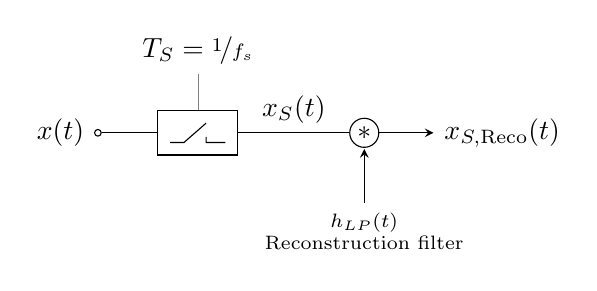
\begin{tikzpicture}
\node [emptypoint,label=left:$x(t)$] (in) {};
\node [box,right=of in,pin=above:{$T_S=\nicefrac{1}{f_s}$}] (switch) {\switch};
\coordinate [right=of switch,label=above:$x_S(t)$] (helper);
\node [round, right=of helper] (convolution) {$\ast$};
\coordinate [right=of convolution,label=right:$x_{S,\text{Reco}}(t)$] (out);
\node [below=of convolution] (lp-ir)
  {\twolines{$h_{LP}(t)$}{Reconstruction filter}};
\path [arrow] (lp-ir) -- (convolution);

\path [noarrow] (in) -- (switch) (switch) -- (convolution);
\path [arrow] (convolution) -- (out);
\end{tikzpicture}

\end{document}
